\documentclass[12pt, a4paper]{article}
    \usepackage[utf8]{inputenc}
    %\usepackage[english, spanish]{babel}
    %\usepackage{fullpage} % changes the margin
    \usepackage{graphicx} 
    \usepackage{enumitem} 
    \usepackage{chngcntr}
    \counterwithin{figure}{section}
    \renewcommand{\thesection}{\arabic{section}} 
    \renewcommand{\thesubsection}{\thesection.\arabic{subsection}}
    \renewcommand{\baselinestretch}{1.5}

    \usepackage{amsmath}
    \usepackage{mathptmx}
    \usepackage[spanish, es-tabla]{babel}
    \usepackage{amssymb}
    \usepackage{makeidx}
    \usepackage{float}
    \pagenumbering{arabic}
    \usepackage[left=25mm, right=25mm, top=25mm, bottom=25mm]{geometry}

    \usepackage[backend=biber]{biblatex}
    \bibliography{referencias}

\begin{document}

    \begin{titlepage}
        \centering
        {\scshape\Large Universidad Central de Venezuela \par}
        {\scshape\Large Facultad de ingeniería \par}
        {\scshape\Large Escuela de ingeniería Eléctrica \par}
        {\scshape\Large Departamento de Electrónica, Computación y Control \par}

        \vspace{6cm}
        {\Large\bfseries LABORATORIO 5 - Polarización del JFET\par}
        \vspace{6cm}

        \vfill
        %\begin{flushleft}
        %    Auxiliar docente:\par
        %    Tovar José
        %\end{flushleft}
        %\vspace{-2cm} %pendiente
        \begin{flushright}
            Estudiantes:\par
            Santana Ricardo C.I.:29571461 \par
            Fajardo Carla C.I.:27571576
            \vspace{1cm}  
        \end{flushright}
        \vfill
        {\large Febrero, 2024 \par}
    \end{titlepage}

    \tableofcontents

    \newpage

    \section{Resumen}

    La presente practica de laboratorio consistió en medir la tensión de cada uno de los puertos de un JFET para así poder hallar el punto estático de operaciones, luego con un potenciómetro se comenzó a variar la resistencia que se encontraba conectada a la fuente (source) hasta conseguir diversos puntos estáticos de operaciones y así poder ver las distintas formas de polarización del JFET utilizado. Es importante destacar que la resistencia $R_D$ requerida en la práctica era de 6.2k$\Omega$, sin embrago, se utilizó dos resistencia en serie que fueran aproximadamente equivalente. 
    
    \newpage

    \section{Introducción}

    Existen diversos tipos de transistores con distintas aplicaciones, de los cuales cabe señalar el transistor de efecto de campo (FET), el cual controla la corriente que circula por uno de sus pines a través del voltaje aplicado entre sus otros dos terminales, a diferencia del BJT que controla la corriente respecto a otra corriente; por tal motivo el FET suele utilizarse en los circuitos como amplificador y como interruptor.

    Sin importar el tipo de FET, sea canal N o canal P, cuenta con tres terminales denominados puerta (Gate), drenador (Drain) y surtidor (Source). Cada uno cuenta con su característica de transferencia específicas y datos particulares que permitiran polarizar el transistor y operarlo en la zona deseada, las más comunes son el voltaje de Pinch-Off y la corriente de dreandor con $V_{GS} = 0$. 

    \newpage

    \section{Objetivos}
    
    \subsection{Objetivo General}
    \begin{itemize}
        \item Analizar el modo de operacion de un transistor JFET canal n. 
    \end{itemize}

    \subsection{Objetivos Específicos}
    \begin{itemize}
        \item Estudiar la polarización de un JFET de canal n.
        \item Reconocer y trabajar con la característica de transferencia y la característica de salida de un JFET de canal n.
    \end{itemize}

    \newpage

    \section{Marco Teórico}

    El transistor de efecto de campo FET (Field Effect Transistor), es un dispositivo semiconductor de portadores mayoritarios, de tres terminales, cuya operación depende de la aplicación de un campo eléctrico para el control de las corrientes, esto es, el FET es una fuente de corriente controlada por tensión.Los FET pueden plantearse como resistencias controladas por diferencia de potencial. Tienen tres terminales, denominadas Puerta (gate), Drenador (drain) y Fuente (source). La puerta es la terminal equivalente a la base del BJT. El transistor de efecto de campo se comporta como un interruptor controlado por tensión, donde el voltaje aplicado a la puerta permite hacer que fluya o no corriente entre drenador y fuente.Así como los transistores bipolares se dividen en NPN y PNP, los de efecto de campo o FET son también de dos tipos: canal N y canal P.

    \begin{figure}[h!]
        \centering
        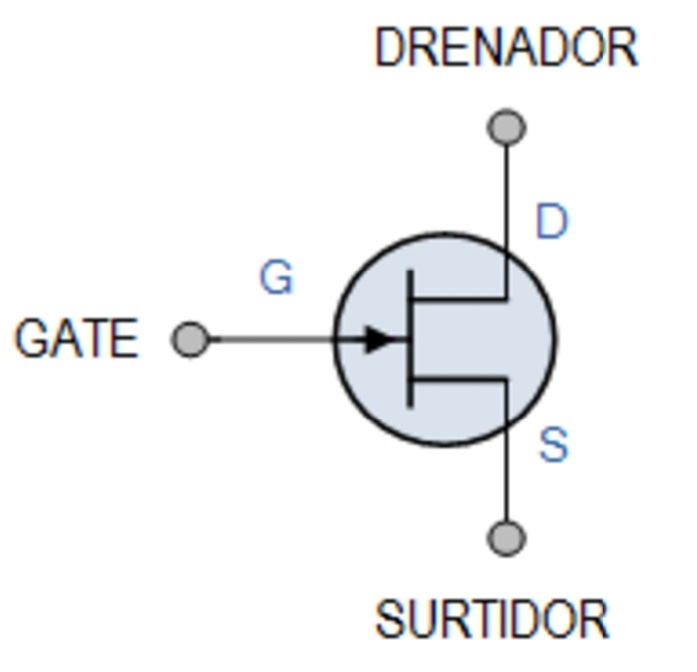
\includegraphics[height=5cm\textwidth]{fetn.jpg}
        \caption{Transistor FET canal n}
        \label{fig:t1}
    \end{figure}

    \begin{figure}[h!]
        \centering
        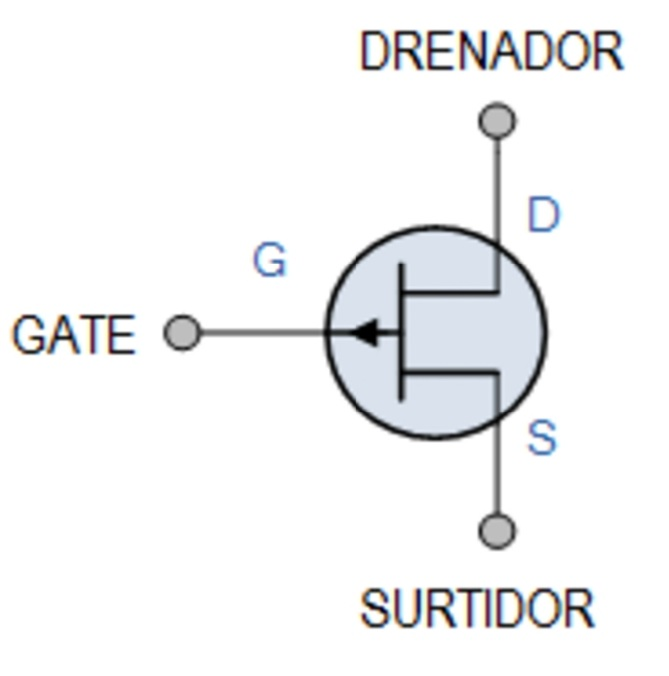
\includegraphics[height=5cm\textwidth]{fetp.jpg}
        \caption{Transistor FET canal p}
        \label{fig:t2}
    \end{figure}

    \subsection{Polarización FET}

    El modo normal de polarización de un FET de canal N requiere que la tensión entre puerta y fuente sea negativa ($V_{GS} < 0$) mientras que la tensión entre Drenador y Fuente tiene que ser positiva ($V_{DS} > 0$).

    \begin{figure}[h!]
        \centering
        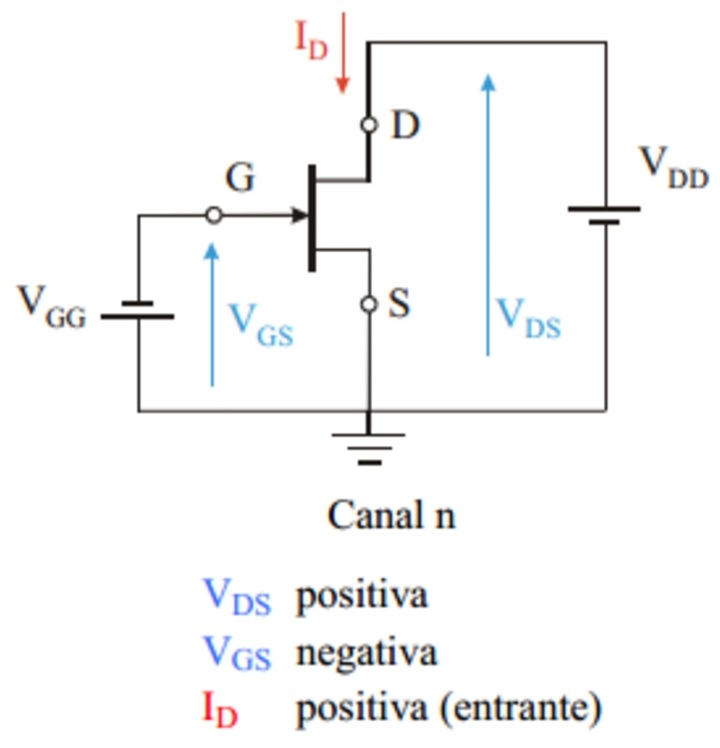
\includegraphics[height=5cm\textwidth]{polarizacionfet.jpg}
        \caption{Polarización del FET}
        \label{fig:t3}
    \end{figure}

    \subsection{Tipos de transistores de efecto de campo FET.}

    Hay muchas formas de definir los diferentes tipos de FET disponibles. Los diferentes tipos significan que, durante el diseño del circuito electrónico, hay una elección del componente electrónico adecuado para el circuito. Al seleccionar el dispositivo correcto, es posible obtener el mejor rendimiento para el circuito dado.
    
    Los FET pueden clasificarse de varias formas. Hay muchos tipos diferentes de FET en el mercado para los que existen varios nombres. Algunas de las categorías principales son:

    \begin{itemize}
        \item JFET
        \item MOSFET
    \end{itemize}

    \subsection{Transistor JFET.}

    El transistor de efecto de campo de unión o JFET es un dispositivo semiconductor unipolar de tres terminales.

    Es básicamente una barra semiconductora N o P (canal), en unión con otros dos semiconductores contrarios al tipo del canal. Si el canal es de semiconductor N, los otros 2 semiconductores serán P o si el canal es de semiconductor P, los otros 2 semiconductores serán N. Tiene 3 contactos unidos a los semiconductores por contactos óhmicos, El drenador (D) y la fuente (F) en los extremos del canal, y otra patilla llamada Puerta o Gate (G)en uno de los otros 2 semiconductores.

    \subsection{Estructura del JFET}

    La ruta de corriente entre estos dos terminales (fuente y drenador) se denomina "canal", que puede estar hecho de un material semiconductor tipo P o tipo N.

    \begin{itemize}
        \item Si el canal es del tipo semiconductor N se llama JFET de canal N (las otras patitasas serán P).
        \item Si el canal es del tipo semiconductor P se llaman JFET de canal P (las otras patillas serán N).
    \end{itemize}

    \subsection{Funcionamiento del JFET}

    En un JFET de canal N tenemos una 2 uniones PN entre el gate (G), que es semiconductor P y la fuente (N) que es el canal y la otra entre el otro semiconductor P y el canal. Si esta unión PN la polarizamos inversamente, la unión PN entre G y el canal tenemos la tensión $V_{GS}$. 
    
    Al aumentar esta tensión aumentará la zona de agotamiento y por lo tanto disminuirá el ancho del canal, lo que hace que tendrá más resistencia al paso de la corriente. La zona de agotamiento a veces también se llama zona de deplexión. Si disminuye el canal, la corriente entre el drenador (D) y la fuente (S) disminuye.

    \subsection{Voltaje de “pinch off” }

    El voltaje de Pinch off es el voltaje que se aplica a la puerta o compuerta de un transistor JFET para estrangular el canal y reducir la corriente de drenaje a un nivel muy bajo. El voltaje de Pinch off también determina la transición del transistor de la región lineal a la región de saturación, donde el transistor actúa como una fuente de corriente constante. El voltaje de Pinch off depende del tipo y las dimensiones del canal.

    \subsection{Regiones de operación del JFET}

    \subsubsection{JFET en región de corte}

    En esta región la intensidad entre drenador y fuente es nula (ID=0). En este caso, la tensión entre puerta y fuente es suficientemente negativa que las zonas de inversión bloquean y estrangulan el canal cortando la corriente entre drenador y fuente.

    En las hojas técnicas se denomina a esta tensión como de estrangulamiento o pinch-off y se representa por VGS (off) o Vp.

    \subsubsection{JFET en región lineal}

    En esta región, el JFET se comporta como una resistencia no lineal que es utilizada en muchas aplicaciones donde se precise una resistencia variable controlada por tensión.

    \subsubsection{JFET en región de saturación}

    En esta región, de similares características que un BJT en la región lineal, el JFET tiene unas características lineales que son utilizadas en amplificación.

    Se comporta como una fuente de intensidad controlada por la tensión VGS cuya ID es prácticamente independiente de la tensión VDS. La ecuación que relaciona la ID con la VGS se conoce como ecuación cuadrática o ecuación de Schockley que viene dada por

    $$I_D = I_{DSS}\left( 1-{V_{GS} \over V_P}\right) ^2$$

    donde $V_p$ es la tensión de estrangulamiento y la $I_{DSS}$ es la corriente de saturación. Esta corriente se define como el valor de $I_D$ cuando $V_{GS}=0$, y esta característica es utilizada con frecuencia para obtener una fuente de corriente de valor constante ($I_{DSS}$).

    Esta relación junto a las características del JFET permiten obtener gráficamente el punto estático de operaciones Q del transistor en la región de saturación. La figura 4 muestra la representación gráfica de este punto Q y la relación existente en ambas curvas, la característica de transferencia y, las cuales permiten determinar el punto de polarización de un transistor utilizando métodos gráficos.

    \begin{figure}[h!]
        \centering
        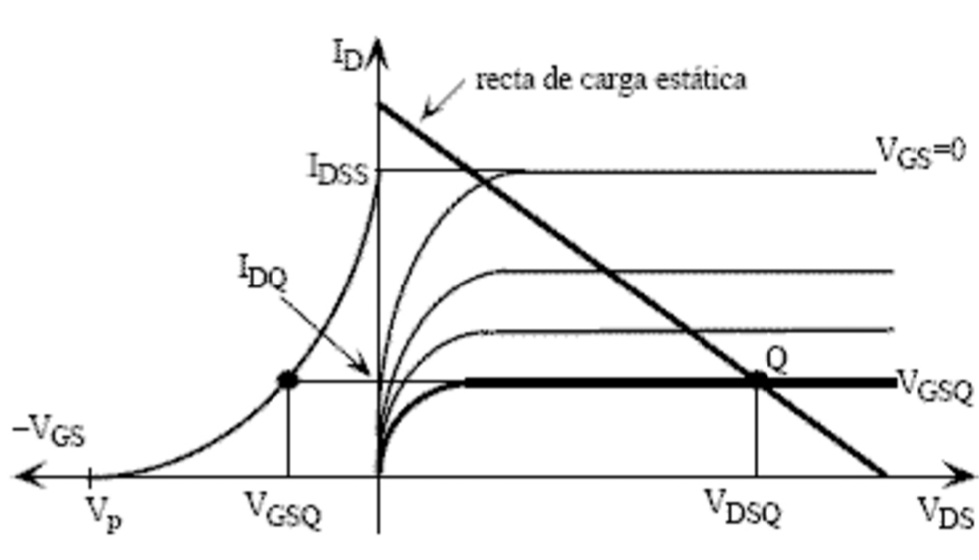
\includegraphics[height=5cm\textwidth]{curvafet.jpg}
        \caption{Curva característica de transferencia y el punto de operaciones Q}
        \label{fig:t4}
    \end{figure}

    \subsubsection{FET en región de ruptura}

    Una tensión alta en los terminales del JFET puede producir ruptura por avalancha a través de la unión de puerta. Las especificaciones de los fabricantes indican la tensión de ruptura entre drenaje y fuente con la puerta cortocircuitada con la fuente; esta tensión su valor está comprendido entra 20 y 50V. Las tensiones de polarización nunca deben superar estos valores para evitar que el dispositivo se deteriore.

    \newpage

    \section{Metodología}

    \subsection{Trabajo Previo al Laboratorio}

    \begin{enumerate}
        \item \label{p11}	Se determinó el punto estático de operación para el circuito de la Figura \ref{fig:cir1}. Para el valor de $I_{DSS}$ y Vp, se obtuvo del manual del fabricante según el transistor a utilizar.
        \item \label{p12}	Se obtuvo la tensión en cada uno de los terminales del JFET: tensión en el Drenador ($V_D$), tensión en la Puerta ($V_G$) y la tensión en el Surtidor ($V_S$).
    \end{enumerate}

    \begin{figure}[h!]
        \centering
        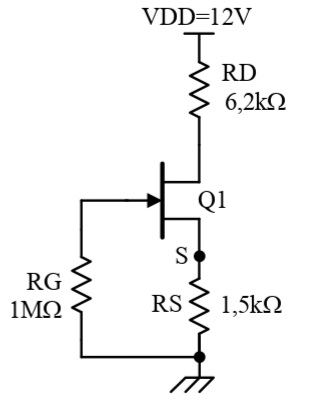
\includegraphics[height=5cm\textwidth]{circuito1.jpg}
        \caption{Polarización del JFET canal n.}
        \label{fig:cir1}
    \end{figure}

    \subsection{Trabajo de Laboratorio}

    \begin{enumerate}
        \item \label{p21}	Para el circuito de la Figura \ref{fig:cir1}, se midió la tensión en el Drenador (VD), tensión en la Puerta ($V_G$) y la tensión en el Surtidor ($V_S$). Se determinó el punto estático de operación: la tensión Drenador-Surtidor ($V_D$S) haciendo $V_D-V_S$ de los valores medidos y la corriente de Drenador ($I_D$) de manera indirecta haciendo $(V_{DD}-V_D)/R_D$; para RD se empleó su valor nominal.
        \item \label{p22}	Para el circuito de la Figura \ref{fig:cir2}, se varió el potenciómetro de hasta conseguir el punto de estático de operación. Anote las mediciones.
        \item \label{p23} 	Se varió el potenciómetro hacia un sentido para conseguir una variación de $0.1V$ en la tensión del Drenador ($V_D$) con respecto al medido en el punto \ref{p22}, se anotó el valor y se midió la tensión en los otros terminales del transistor.
        \item \label{p24} 	Se siguió variando el potenciómetro en el mismo sentido que el punto \ref{p23} para obtener variaciones de 0.1V en la tensión del Drenador (VD) hasta llegar al extremo del potenciómetro. En cada variación se midió las tensiones en cada uno de los terminales del transistor. Realice una tabla.
    \end{enumerate}

    \begin{figure}[h!]
        \centering
        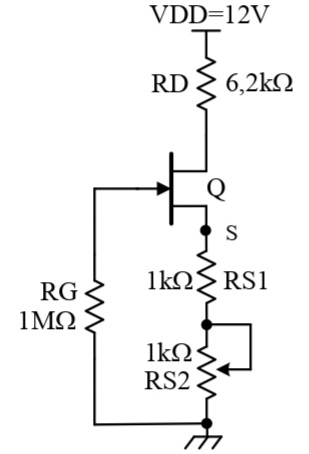
\includegraphics[height=5cm\textwidth]{circuito2.jpg}
        \caption{Variación en la Polarización del JFET.}
        \label{fig:cir2}
    \end{figure}

    \newpage

    \section{Cálculos prévios}

    Se trabajará con el transistor FET canal n 2N5555, el cual posee las siguientes especificaciones:
    
    \begin{table}[h!]
        \centering
        \caption{Características del transistor 2N5555} %nombre de la tabla
        \label{tab:5555} %indice de la tabla
        \begin{tabular}{c}
            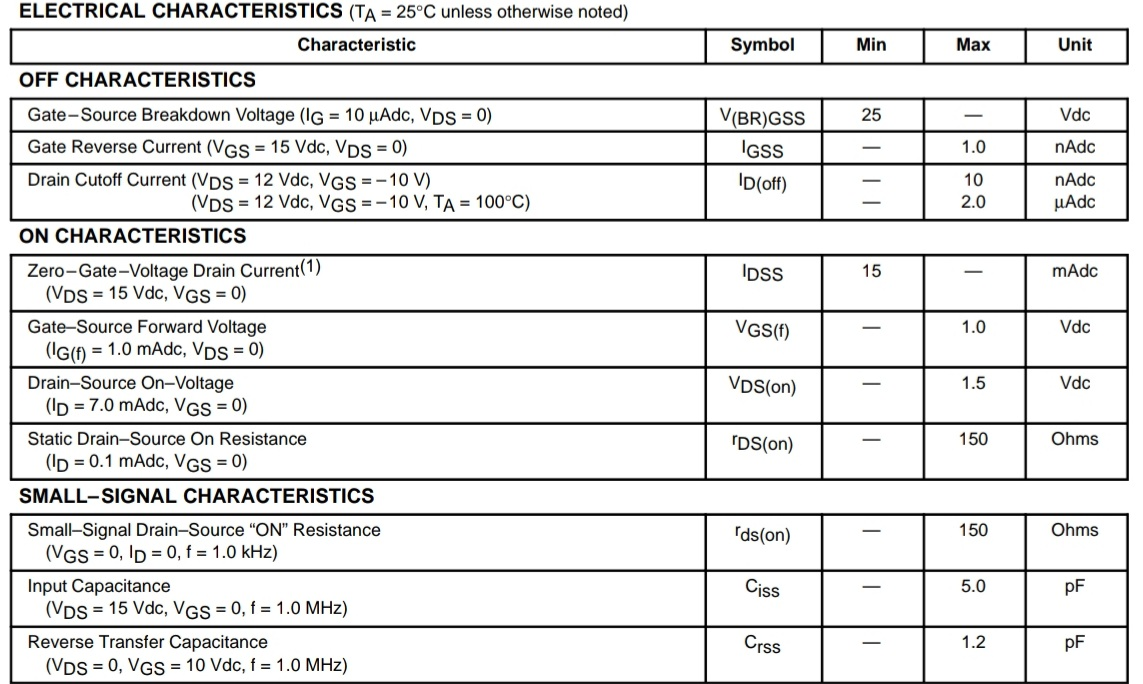
\includegraphics[width=16cm\textwidth]{2N5555.jpg} \\
        \end{tabular}
    \end{table}
    
    de las cuales se deduce por promediación que:

    $V_P = -1V$

    $I_{DSS} = 15mA$

    Entonces analizando el circuito de la figura \ref{fig:cir1}, para encontrar el punto estático de operación $Q(V_{DSQ},I_{DQ})$, donde los condensadores se desacoplan por estar trabajando en DC.

    \begin{figure}[h!]
        \centering
        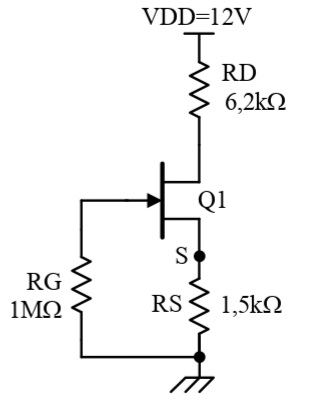
\includegraphics[height=5cm\textwidth]{circuito1.jpg} \par
        Figura \ref{fig:cir1}. Polarización del JFET canal n.
    \end{figure}

    Se tiene un JFET autopolarizado. Esto es debido a que la corriente circulando por $R_G$ es cero y, por tanto, toda la corriente ($I_D$) que entra por el drenador D sale por la fuente S.

    Analizando la malla relacionada al circuito de la compuerta con $I_G = 0$,

    $$V_{GS} = -I_DR_S \rightarrow I_D = -{V_{GS} \over R_S}$$

    \begin{equation} \label{eq1}
        I_D = -{V_{GS} \over R_S}
    \end{equation}

    Conociendo la características de transferencia de un JFET que relaciona $V_{GS}$ e $I_D$ por la fórmula \eqref{eqvgs}

    \begin{equation} \label{eqvgs}
        I_D = I_{DSS}\left( 1-{V_{GS} \over V_P}\right) ^2
    \end{equation}

    Entonces

    $$I_{DQ} = I_{DSS}\left( 1-{V_{GSQ} \over V_P}\right) ^2 = -{V_{GSQ} \over R_S}$$

    buscando $V_{GSQ}$
    
    \begin{equation}
        \label{eq3}
        \begin{split}
            I_{DSS}\left( 1-{V_{GSQ} \over V_P}\right) ^2  & = -{V_{GSQ} \over R_S} \\
            1 - 2{V_{GSQ} \over V_P} + ({V_{GSQ} \over V_P})^2  & = -{V_{GSQ} \over I_{DSS}R_S} \\
            1 - 2{V_{GSQ} \over V_P} + {V_{GSQ}^2 \over V_P^2} + {V_{GSQ} \over I_{DSS}R_S} & = 0 \\
            {1 \over V_P^2}V_{GSQ}^2 + \left({1 \over I_{DSS}R_S} - {2 \over V_P}\right)V_{GSQ} + 1 & = 0 \\
        \end{split}
    \end{equation}

    Reemplazando valores conocidos en \eqref{eq3} y resolviendo ecuación de segundo grado

    \begin{split}
        {1 \over V_P^2}V_{GSQ}^2 + \left({1 \over I_{DSS}R_S} - {2 \over V_P}\right)V_{GSQ} + 1 & = 0 \\
        {1 \over (-1V)^2}V_{GSQ}^2 + \left({1 \over (15mA)(1.5k\Omega)} - {2 \over (-1V)}\right)V_{GSQ} + 1 & = 0 \\
        V_{GSQ}^2 + {92 \over 45}V_{GSQ} + 1 & = 0 \\
    \end{split}

    $$V_{GSQ} = -0.81V$$

    \begin{figure}[h!]
        \centering
        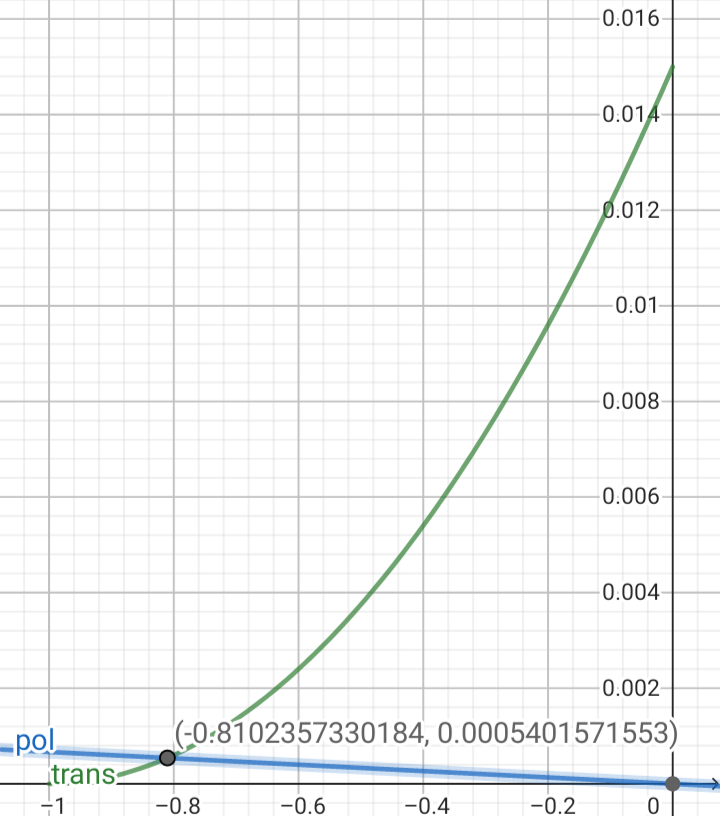
\includegraphics[height=5cm\textwidth]{grafQ.png}
        \caption{Intersección de las ecuaciones de recta de polarización \eqref{eq1} y característica de transferencia V_{GS} vs I_D \eqref{eqvgs}}
        \label{fig:vgsq}
    \end{figure}

    Sustiyendo en \eqref{eq1}

    $$I_{DQ} = -{V_{GSQ} \over R_S} = -{(-0.8V) \over 1.5k\Omega} = 0.533mA$$

    Analizando malla relacionada al drenador

    $$V_{DD} = I_DR_D + V_{DS} + I_DR_S$$

    Particularizando para calcular $V_{DSQ}$

    \begin{equation}
        \label{eq4}
        \begin{split}
            V_{DD} & = I_{DQ}R_D + V_{DSQ} + I_{DQ}R_S \\
            I_{DQ}R_D + V_{DSQ} + I_{DQ}R_S & = V_{DD} \\
            V_{DSQ} & = V_{DD} - I_{DQ}(R_D + R_S)
        \end{split}
    \end{equation}
    
    Reemplazando valores en \eqref{eq4}

    $$V_{DSQ} = 12V - 0.533mA(6.2 + 1.5)k\Omega = 7.89V$$

    Punto de operacion

    $$Q : (7.89V, 0.533mA)$$

    Entonces el transistor se encuentra en zona de saturación
    
    Como $I_G = 0$, entonces no hay caida de tensión en $R_G$ y $V_G = 0$

    $V_S = - V_{GS} = 0.81V$

    $V_{DS} = V_D - V_S \rightarrow V_D = V_{DS} + V_S = 7.89V + 0.81V = 8.7V$

    \begin{table}[h!]
        \centering
        \caption{Voltajes teoricos en Puerta, Drenador y Fuente}
        \label{tab:vteorico} 
        \begin{tabular}{|c|c|c|} \hline
            V_G [V] & V_D [v] & V_S [v] \\ \hline
            0 & 8.7 & 0.81 \\ \hline
        \end{tabular}
    \end{table}

    \newpage

    \section{Materiales e Instrumentos}

    \begin{table}[h!]
        \centering
        \caption{Equipos o instrumentos}
        \label{tab:instrumentos}
        \begin{tabular}{|c|c|c|} \hline
            Equipo                    &  Marca&    Modelo   \\ \hline
            Osciloscopio              &  UNI-T & UTD2102CEX+ \\ 
            Fuente de alimentacion DC  &  UNI-T & UTP3305-II  \\ \hline
        \end{tabular}
    \end{table}

    \begin{table}[h!]
        \centering
        \caption{Componentes y materiales}
        \label{tab:componentes}
        \begin{tabular}{|c|c|c|} \hline
            Referencia&Descripción&    Especificaciones   \\ \hline
                  RD1 = 2.7k$\Omega$   & Resistencia   &          1/4 W         \\
                  RD2 = 3.6k$\Omega$   & Resistencia   &          1/4 W         \\
                  RG = 1M$\Omega$   & Resistencia &  1/4 W         \\
                  RS =  1.5k$\Omega$  &Resistencia  &         1/4 W         \\
                  RS1 = 1k$\Omega$   &Resistencia   &         1/4 W         \\
                  RS2 = 1k$\Omega$             &Potenciómetro Preset&  \\
            Q = 2N5555  &Tansistor JFET canal n &   \\ \hline
            \end{tabular}
            
    \end{table}

    \newpage

    \section{Presentación de Resultados}

    \begin{table}[h!]
        \centering
        \caption{Tensiones en los terminales del transistor, prueba \ref{p21}}
        \label{tab:Q1}
        \begin{tabular}{|c|c|c|c|c|c|} \hline
            $V_D$ [V]  &  $V_S$ [V] &  $V_G$ [V]  &  $I_D$ [A] & $V_{DS}$ [V] & zona \\ \hline
            2.6 ± 0.1  &  2.2 ± 0.1 &  0.000 ± 0.002  &  0.001492 \pm 0.000324  &  0.4 \pm 0.2  & ohmica \\ \hline
        \end{tabular}
    \end{table}

    \begin{table}[h!]
        \centering
        \caption{Tensiones en los terminales del transistor, prueba \ref{p22}}
        \label{tab:Q2}
        \begin{tabular}{|c|c|c|c|c|c|} \hline
            $V_D$ [V]  &  $V_S$ [V] &  $V_G$ [V]  &  $I_D$ [A] & $V_{DS}$ [V] & zona \\ \hline
            2.6 ± 0.1  &  2.2 ± 0.1 &  0.000 ± 0.002  &  0.001492 \pm 0.000324  &  0.4 \pm 0.2  & ohmica \\ \hline
        \end{tabular}
    \end{table}

    \begin{table}[h!]
        \centering
        \caption{Tensiones en los terminales del transistor, prueba \ref{p23} y \ref{p24}}
        \label{tab:QP}
        \begin{tabular}{|c|c|c|c|c|c|} \hline
            $V_D$ [V]  &  $V_S$ [V] &  $V_G$ [V]  &  $I_D$ [A] & $V_{DS}$ [V] & zona \\ \hline
            2.7 ± 0.1  &  2.2 ± 0.1 &  0.000 ± 0.002  &  0.001476 \pm 0.000322  &  0.5 \pm 0.2  & ohmica \\
            2.8 ± 0.1  &  2.4 ± 0.1 &  0.000 ± 0.002  &  0.001460 \pm 0.000321  &  0.4 \pm 0.2  & ohmica \\
            2.9 ± 0.1  &  2.4 ± 0.1 &  0.000 ± 0.002  &  0.001444 \pm 0.000319  &  0.5 \pm 0.2  & ohmica \\
            3.0 ± 0.1  &  2.5 ± 0.1 &  0.000 ± 0.002  &  0.001429 \pm 0.000317  &  0.5 \pm 0.2  & ohmica \\
            3.1 ± 0.1  &  2.6 ± 0.1 &  0.000 ± 0.002  &  0.001413 \pm 0.000316  &  0.5 \pm 0.2  & ohmica \\
            3.2 ± 0.1  &  2.8 ± 0.1 &  0.000 ± 0.002  &  0.001397 \pm 0.000314  &  0.4 \pm 0.2  & ohmica \\
            3.3 ± 0.1  &  2.8 ± 0.1 &  0.000 ± 0.002  &  0.001381 \pm 0.000313  &  0.5 \pm 0.2  & ohmica \\
            3.4 ± 0.1  &  2.8 ± 0.1 &  0.000 ± 0.002  &  0.001365 \pm 0.000311  &  0.6 \pm 0.2  & ohmica \\ \hline
        \end{tabular}
    \end{table}

    {\bf Observación:} Para el cáculo del punto de operacion se utilizan las fórmulas \eqref{Qeq1}, \eqref{Qeq2}, \eqref{Qeq3} y \eqref{Qeq4} en los anexos.

    \newpage

    A continuación se muestra la característica de transferencia relacionada a las figuras \ref{fig:cir1} y \ref{fig:cir2} con mediciones que establecieron el punto de operación en las tablas \ref{tab:Q1} y \ref{tab:Q2}.

    \begin{figure}[h!]
        \centering
        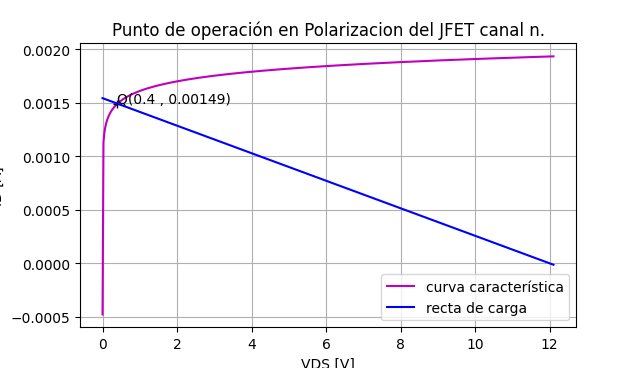
\includegraphics[height=6cm\textwidth]{pol.png}
        \caption{Curva Característica, recta de carga y punto de operación del circuito de la figura \ref{fig:cir1}}
        \label{fig:pol}
    \end{figure}

    \begin{figure}[h!]
        \centering
        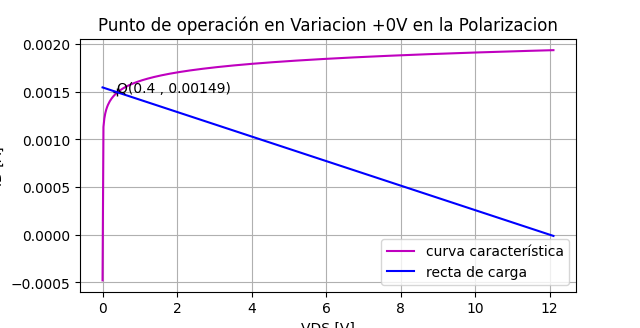
\includegraphics[height=6cm\textwidth]{var00.png}
        \caption{Curva Característica, recta de carga y punto de operación del circuito de la figura \ref{fig:cir2}}
        \label{fig:v0}
    \end{figure}

    \newpage

    \subsection{Resultados en la variación de potenciometro $R_{S2}$}

    \begin{table}[h!]
        \centering
        \caption{Tensiones en los terminales de transistor y punto de operación para $V_D+0.1$ [V]}
        \label{tab:v1}
        \begin{tabular}{|c|c|c|c|c|c|} \hline
            $V_D$ [V]  &  $V_S$ [V] &  $V_G$ [V]  &  $I_D$ [A] & $V_{DS}$ [V] & zona \\ \hline
            2.7 ± 0.1  &  2.2 ± 0.1 &  0.000 ± 0.002  &  0.001476 \pm 0.000322  &  0.5 \pm 0.2  & ohmica \\ \hline
        \end{tabular}
    \end{table}

    \begin{figure}[h!]
        \centering
        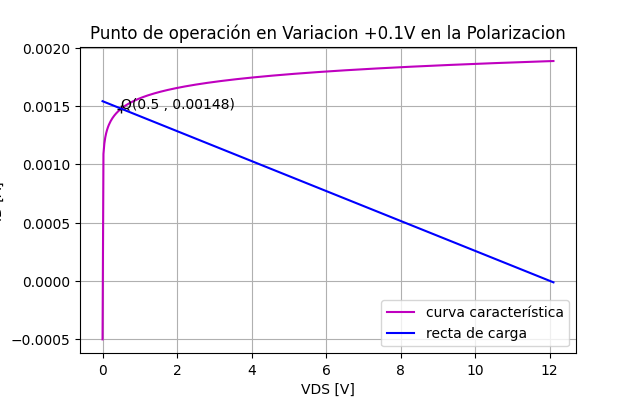
\includegraphics[height=5cm\textwidth]{var01.png}
        \caption{Curva Característica, recta de carga y punto de operación para $V_D+0.1$ [V]}
        \label{fig:v1}
    \end{figure}

    \begin{table}[h!]
        \centering
        \caption{Tensiones en los terminales de transistor y punto de operación para $V_D+0.2$ [V]}
        \label{tab:v2}
        \begin{tabular}{|c|c|c|c|c|c|} \hline
            $V_D$ [V]  &  $V_S$ [V] &  $V_G$ [V]  &  $I_D$ [A] & $V_{DS}$ [V] & zona \\ \hline
            2.8 ± 0.1  &  2.4 ± 0.1 &  0.000 ± 0.002  &  0.001460 \pm 0.000321  &  0.4 \pm 0.2  & ohmica \\ \hline
        \end{tabular}
    \end{table}

    \begin{figure}[h!]
        \centering
        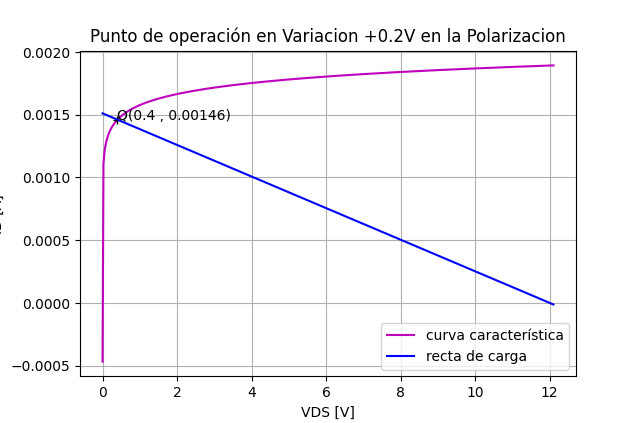
\includegraphics[height=5cm\textwidth]{var02.png}
        \caption{Curva Característica, recta de carga y punto de operación para $V_D+0.2$ [V]}
        \label{fig:v2}
    \end{figure}

    \newpage

    \begin{table}[h!]
        \centering
        \caption{Tensiones en los terminales de transistor y punto de operación para $V_D+0.3$ [V]}
        \label{tab:v3}
        \begin{tabular}{|c|c|c|c|c|c|} \hline
            $V_D$ [V]  &  $V_S$ [V] &  $V_G$ [V]  &  $I_D$ [A] & $V_{DS}$ [V] & zona \\ \hline
            2.9 ± 0.1  &  2.4 ± 0.1 &  0.000 ± 0.002  &  0.001444 \pm 0.000319  &  0.5 \pm 0.2  & ohmica \\ \hline
        \end{tabular}
    \end{table}

    \begin{figure}[h!]
        \centering
        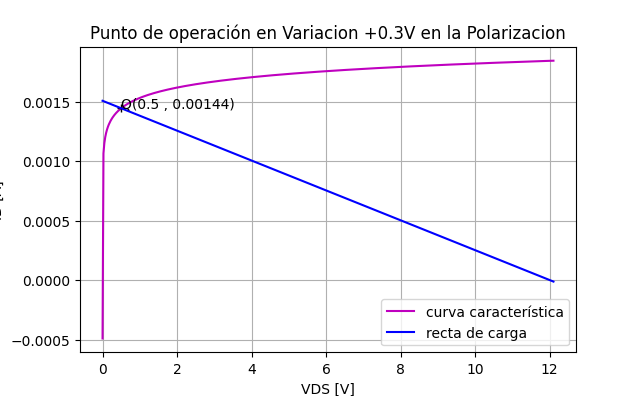
\includegraphics[height=5cm\textwidth]{var03.png}
        \caption{Curva Característica, recta de carga y punto de operación para $V_D+0.3$ [V]}
        \label{fig:v3}
    \end{figure}

    \begin{table}[h!]
        \centering
        \caption{Tensiones en los terminales de transistor y punto de operación para $V_D+0.4$ [V]}
        \label{tab:v4}
        \begin{tabular}{|c|c|c|c|c|c|} \hline
            $V_D$ [V]  &  $V_S$ [V] &  $V_G$ [V]  &  $I_D$ [A] & $V_{DS}$ [V] & zona \\ \hline
            3.0 ± 0.1  &  2.5 ± 0.1 &  0.000 ± 0.002  &  0.001429 \pm 0.000317  &  0.5 \pm 0.2  & ohmica \\ \hline
        \end{tabular}
    \end{table}

    \begin{figure}[h!]
        \centering
        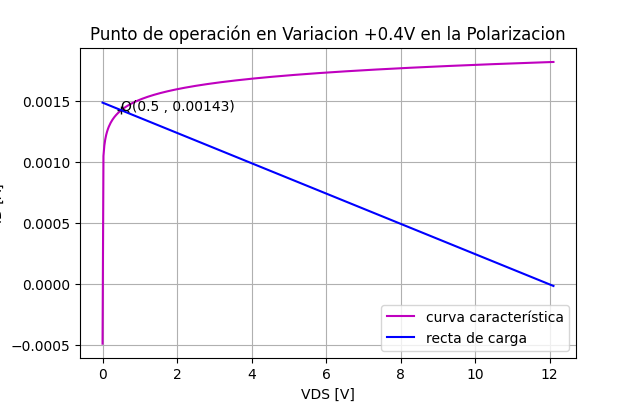
\includegraphics[height=5cm\textwidth]{var04.png}
        \caption{Curva Característica, recta de carga y punto de operación para $V_D+0.4$ [V]}
        \label{fig:v4}
    \end{figure}

    \newpage

    \begin{table}[h!]
        \centering
        \caption{Tensiones en los terminales de transistor y punto de operación para $V_D+0.5$ [V]}
        \label{tab:v5}
        \begin{tabular}{|c|c|c|c|c|c|} \hline
            $V_D$ [V]  &  $V_S$ [V] &  $V_G$ [V]  &  $I_D$ [A] & $V_{DS}$ [V] & zona \\ \hline
            3.1 ± 0.1  &  2.6 ± 0.1 &  0.000 ± 0.002  &  0.001413 \pm 0.000316  &  0.5 \pm 0.2  & ohmica \\ \hline
        \end{tabular}
    \end{table}

    \begin{figure}[h!]
        \centering
        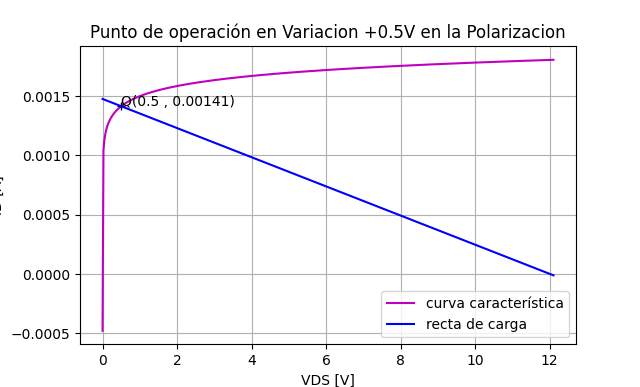
\includegraphics[height=5cm\textwidth]{var05.png}
        \caption{Curva Característica, recta de carga y punto de operación para $V_D+0.5$ [V]}
        \label{fig:v5}
    \end{figure}

    \begin{table}[h!]
        \centering
        \caption{Tensiones en los terminales de transistor y punto de operación para $V_D+0.6$ [V]}
        \label{tab:v6}
        \begin{tabular}{|c|c|c|c|c|c|} \hline
            $V_D$ [V]  &  $V_S$ [V] &  $V_G$ [V]  &  $I_D$ [A] & $V_{DS}$ [V] & zona \\ \hline
            3.2 ± 0.1  &  2.8 ± 0.1 &  0.000 ± 0.002  &  0.001397 \pm 0.000314  &  0.4 \pm 0.2  & ohmica \\ \hline
        \end{tabular}
    \end{table}

    \begin{figure}[h!]
        \centering
        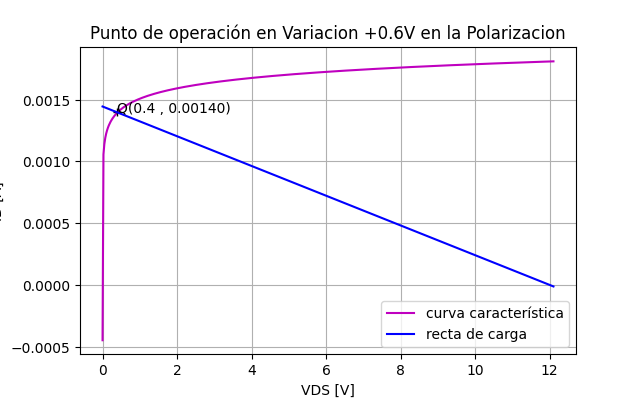
\includegraphics[height=5cm\textwidth]{var06.png}
        \caption{Curva Característica, recta de carga y punto de operación para $V_D+0.6$ [V]}
        \label{fig:v6}
    \end{figure}

    \newpage

    \begin{table}[h!]
        \centering
        \caption{Tensiones en los terminales de transistor y punto de operación para $V_D+0.7$ [V]}
        \label{tab:v7}
        \begin{tabular}{|c|c|c|c|c|c|} \hline
            $V_D$ [V]  &  $V_S$ [V] &  $V_G$ [V]  &  $I_D$ [A] & $V_{DS}$ [V] & zona \\ \hline
            3.3 ± 0.1  &  2.8 ± 0.1 &  0.000 ± 0.002  &  0.001381 \pm 0.000313  &  0.5 \pm 0.2  & ohmica \\ \hline
        \end{tabular}
    \end{table}

    \begin{figure}[h!]
        \centering
        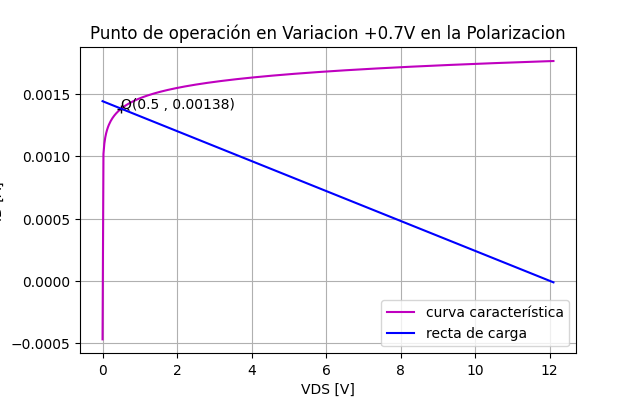
\includegraphics[height=5cm\textwidth]{var07.png}
        \caption{Curva Característica, recta de carga y punto de operación para $V_D+0.7$ [V]}
        \label{fig:v7}
    \end{figure}

    \begin{table}[h!]
        \centering
        \caption{Tensiones en los terminales de transistor y punto de operación para $V_D+0.8$ [V]}
        \label{tab:v8}
        \begin{tabular}{|c|c|c|c|c|c|} \hline
            $V_D$ [V]  &  $V_S$ [V] &  $V_G$ [V]  &  $I_D$ [A] & $V_{DS}$ [V] & zona \\ \hline
            3.4 ± 0.1  &  2.8 ± 0.1 &  0.000 ± 0.002  &  0.001365 \pm 0.000311  &  0.6 \pm 0.2  & ohmica \\ \hline
        \end{tabular}
    \end{table}

    \begin{figure}[h!]
        \centering
        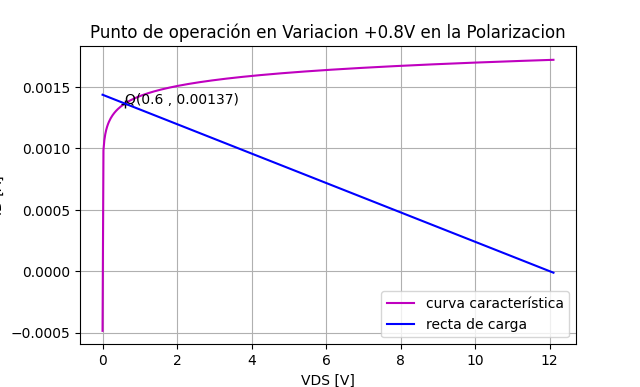
\includegraphics[height=5cm\textwidth]{var08.png}
        \caption{Curva Característica, recta de carga y punto de operación para $V_D+0.8$ [V]}
        \label{fig:v8}
    \end{figure}

    \newpage

    \section{Análisis de Resultados}

    Al realizar las mediciones para el circuito de la figura \ref{fig:cir1} se obtuvo que un VD = 2.6 V; VS = 2.2V  y VG = 0V, además se puede ver que VGS = -2.2 V. Este es un resultado lógico para la polarización del circuito del JFET cana n, ya que es un circuito autopolarizado debido a que la unión compuerta-fuente siempre debe estar polarizada en inversa, sin embargo los valores obtenidos referentes al punto de operación, según la tabla \ref{tab:Q1} son muy alejados a los obtenidos teoricamente en la tabla \ref{tab:vteorico}; incluso se observa que están trabajando en zonas diferentes.

    Al determinar el punto estático de operación para la figura \ref{fig:cir2} obtenemos el mismo que el anterior (0.4V, 1.44mA), se sabe que en la curva característica de salida del JFET se tienen cuatro regiones fundamentales de trabajo, las cuales son: zona óhmica o de no saturación; zona de corriente constante, de saturación o de “pinch off”; zona de ruptura y la zona de corte. Debido al punto de operación obtenido se puede decir que el circuito está en la zona óhmica debido a que para bajas tensiones VDS circula una corriente apreciable ID, esto hace que el JFET se comporte como una resistencia óhmica, esta resistencia entre el terminal del drenador y la fuente está controlada mediante VGS. Si se desea trabajar en zona activa se recomienda reducir la resistencia de drenador, considerando una corriente apropiada para el transistor. Así mismo, se puede decir que en un caso particular el JFET puede comportarse como un interruptor controlado por tensión que puede pasar del estado de conducción a no conducción lo cual dependerá del VGS.
    
    Al observar los gráficos de las figuras \ref{fig:v1} a la \ref{fig:v8}, al variar el potenciómetro hacia un sentido para conseguir variaciones de 0,1V se puede observar que VD aumenta al igual que VS, esto hace que VDS entre las diferentes variaciones sea prácticamente el mismo. Sin embargo, como RS aumenta la ID que es la que circula por el transistor disminuye, por tanto, se puede inferir que al disminuir la resistencia RS con el potenciómetro la corriente que pasa por el transistor aumenta. Se pudo observar que la resistencia RS en el circuito se puede usar para definir VGS sin necesidad de ninguna fuente de tensión adicional, esto es debido a que la corriente que circula por RG es cero y por lo tanto la corriente que entra ID es la que circula por el transistor.


    \newpage
    
    \section{Conclusiones y Recomendaciones}

    Durante la realización de esta práctica se logró consolidar los conocimientos vistos en clase respecto a los transistores JFET canal n autopolarizados, su característica de salida, las diferentes zonas de operación y su característica de transferencia. 

    Con base a los resultados obtenidos se puede decir que debido a la polarización de estos circuitos la resistencia de la fuente controla la corriente del drenador, también altera el voltaje entre el drenador y la fuente y por lo tanto la resistencia en la fuente también puede cambiar el punto estático de operación. 

    En esta práctica se obtuvo que el JFET estaba trabajando en la zona óhmica o de no saturación, en base a esto se puede decir que, así como se mencionó en el análisis, el JFET presenta cuatro regiones de trabajo, cada una de ellas tiene sus ventajas y desventajas, por lo que se observa que al variar la resistencia en la fuente se puede desplazar el punto de operación del transistor a la zona que más nos convenga dependiendo de la utilidad que le vayamos a dar. 

    Por otro lado, es importante mencionar que las experiencias se vieron afectadas por el comportamiento no deseado del transistor 2SK61 el cual era un reemplazo del transistor MPF102, sin embargo, se observó que los valores que se obtenían no eran lógicos con lo que se esperaba, por lo que se tuvo que cambiar al transistor 2N5555 y realizar nuevamente las mediciones. Sin embargo, a pesar de estos inconvenientes, los objetivos de la práctica fueron completados satisfactoriamente.

    \newpage

    \section{Bibliografía}

    \begin{itemize}
        \item Sedra Adel. “Circuitos Microelectrónicos”. En: OXFORD University Press 4 (2002).
        \item Héctor Navarro. “Clases de Transistor de Efecto de Campo”. En (2024). Documento digital. 
    \end{itemize}
    
    \printbibliography

    \newpage

    \section{Anexos}

    \subsection{Cálculo del punto de operación}

    Para los valores $V_{DS}$ y $I_D$ de las tablas \ref{tab:Q1}, \ref{tab:Q2} y \ref{tab:QP} se realizaron los siguientes cálculos:

    Sabiendo que $V_{DD} = 12 \pm 1 [V]$

    \begin{equation}
        V_{DS} = V_D - V_S
        \label{Qeq1}
    \end{equation}

    \begin{equation}
        I_D = \frac{V_{DD} - V_D}{R_D}
        \label{Qeq2}
    \end{equation}

    Para el cálculo de sus respectivas incertidumbres:

    \begin{equation}
        \Delta V_{DS} = \Delta V_D + \Delta V_S
        \label{Qeq3}
    \end{equation}

    \begin{equation}
        \begin{split}
            \Delta I_D & = \left | \frac{\partial I_D}{\partial V_{DD}} \right | \Delta V_{DD} + \left | \frac{\partial I_D}{\partial V_D} \right | \Delta V_D + \left | \frac{\partial I_D}{\partial R_D} \right | \Delta R_D \\
            & = {1 \over R_D} \Delta V_{DD} + {1 \over R_D} \Delta V_D + \frac{V_{DD}-V_D}{R_D^2} \Delta R_D
        \end{split}
        \label{Qeq4}
    \end{equation}

    %\subsection{Cálculo de ganancia}

    \newpage

    Hojas de datos que contienen los valores experimentales recopilados en el laboratorio.

    \begin{figure}[h!]
        \centering
        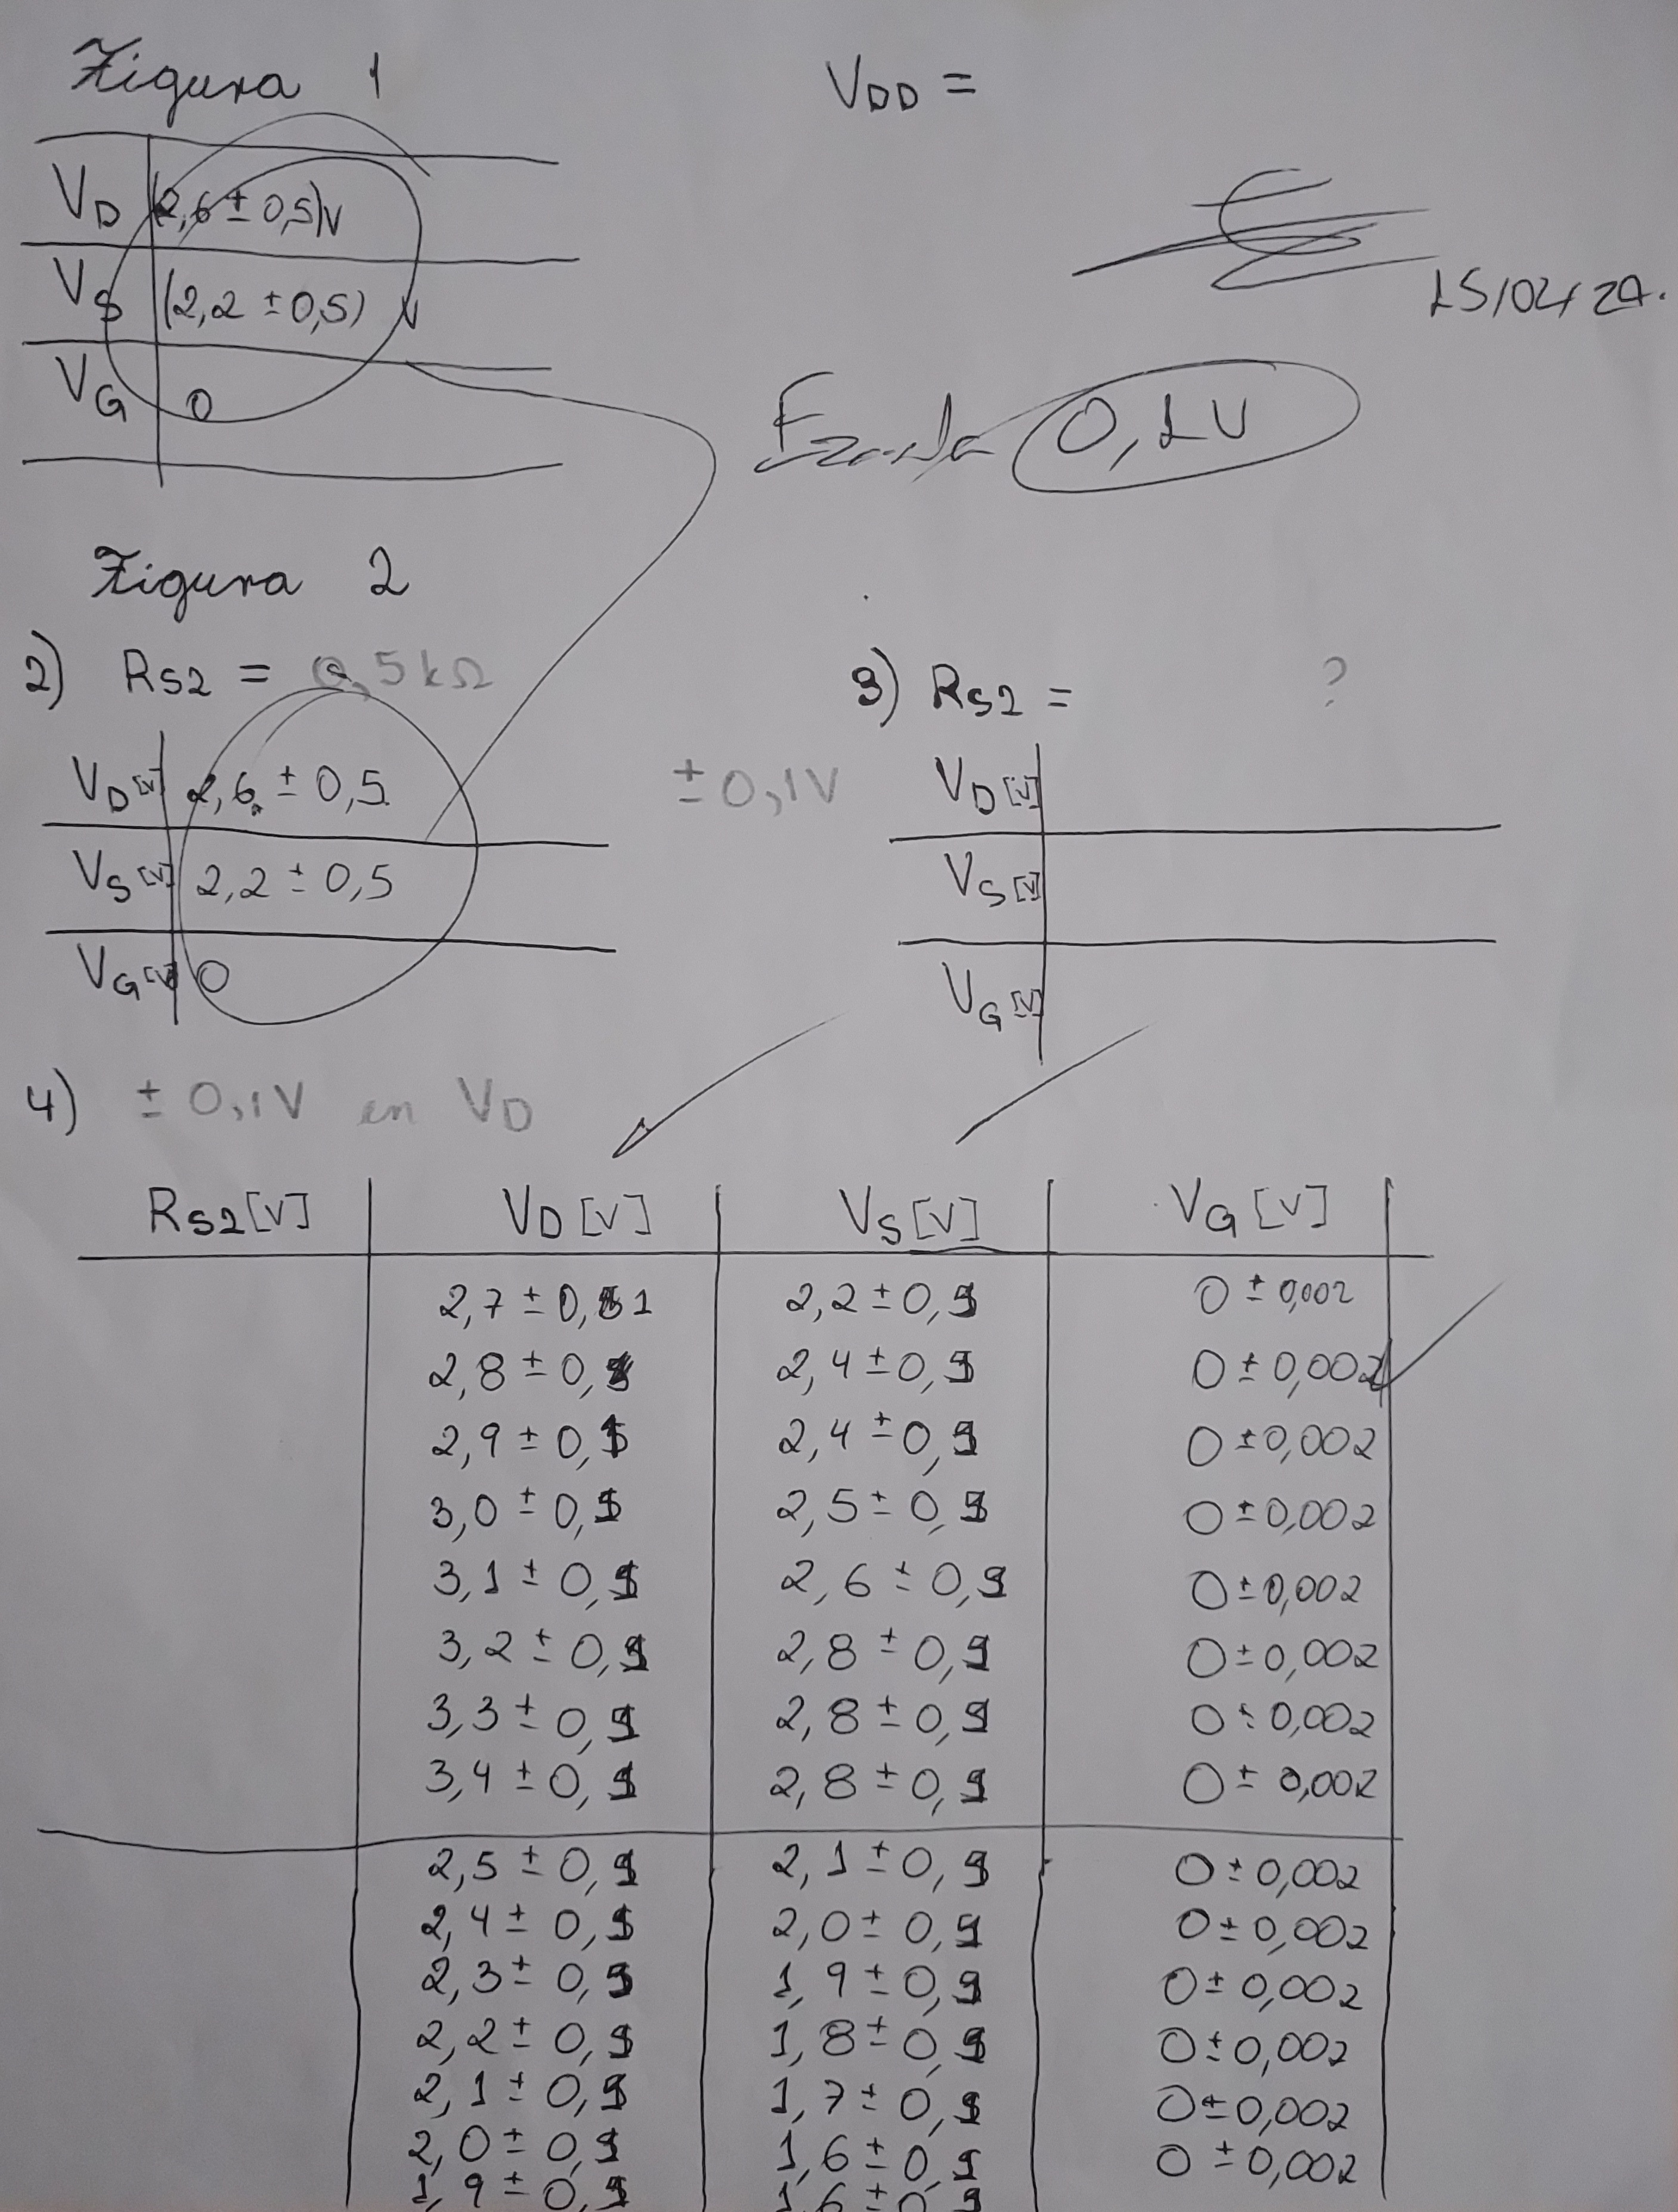
\includegraphics[height=10cm\textwidth]{hd5.jpg}
        \caption{hoja de datos}
        \label{fig:hd5}
    \end{figure}


\end{document}